% report/sections/04_approach.tex -- Part I: synthesis of existing methods into the proposed approach.
\section{From existing methods to the proposed approach}\label{sec:approach}

Five research traditions each solve part of our problem. None answers the question this project
asks: \emph{in this domain, where does the written record stop, and what kind of knowledge is likely
to lie beyond it?} The methods themselves are in \cref{sec:foundations}.

\subsection{What each tradition does well, and where it stops}\label{sec:approach-traditions}

\paragraph{Cognitive task analysis} \evlit{} reaches the decisions, cues and interpretations experts
skip \parencite{schraagen2000cognitive,klein1989critical,hall1995procedural}. \evint{} Every answer
costs expert time, pooling experts multiplies it \parencite{chao1994percentage}, and CTA starts
from the expert, not the written record, so it cannot say where the first interview hour is best
spent.

\begin{figure}[!b]
  \centering
  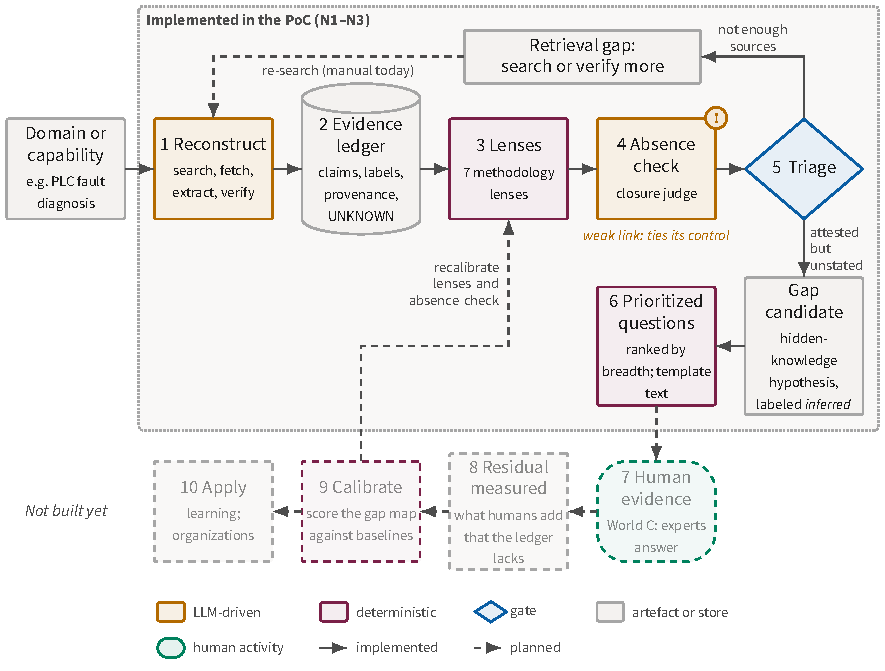
\includegraphics{figures/pdf/fig02_model.pdf}
  \caption[The central model]{What is the whole approach, and which parts exist today? A domain or
    capability enters at the top. Steps 1--6 (solid) are implemented in the PoC: reconstruction,
    evidence ledger, methodology lenses, absence check, triage and questions. Steps 7--9 (dashed)
    are future work: human evidence, calibration and application. Triage splits the output into two
    kinds of gap. A retrieval gap is listed for further search; in the PoC that is a manual re-run,
    since no code feeds it back to reconstruction. Only a gap candidate becomes a hidden-knowledge
    hypothesis (labeled \emph{inferred}) and an expert question. The absence check (step 4) is the
    weak link in the PoC.}
  \label{fig:model}
\end{figure}

\paragraph{LLM research tools} \evlit{} write cited syntheses
\parencite{shao2024assisting,skarlinski2024language,asai2024openscholar} and check atomic claims
against sources \parencite{min2023factscore,rashkin2023measuring,gao2023enabling}, but inherit the
reporting bias of text \parencite{gordon2013reporting,paik2021world}, and their citations often do
not fully support the statements \parencite{liu2023evaluating,venkit2025deeptrace,wu2025automated}.
\evint{} A cited synthesis has no place to record \enquote{searched and found nothing}.

\paragraph{Knowledge management} \evlit{} separates tacit from explicit knowledge
\parencite{nonaka1994dynamic} and codifying from connecting people \parencite{hansen1999whats};
\evint{} the split is a category or a strategy, not a measurement per task.

\paragraph{Requirements engineering and instructional-text NLP} \evlit{} flag terms and relations a
specification lacks relative to its inputs \parencite{ferrari2014measuring}. They predict likely
omissions with a masked language model \parencite{luitel2024improving} and use interview ambiguity as
a cue to tacit knowledge \parencite{ferrari2016ambiguity}. \textcite{torre2020ai} check GDPR privacy policies
against a conceptual model of the content the regulation requires, and report which required types
are absent. NLP work on wikiHow finds implicit and underspecified phrases, with later human edits as
gold \parencite{anthonio2020wikihowtoimprove,anthonio2022clarifying}. \evint{} Each works on one
document or interview against a reference that fixes the missing types in advance. None predicts
knowledge held only by practitioners or routes it to an elicitation channel.

\paragraph{Gap finding in literature} \evlit{} maps \enquote{structured absences} in papers
\parencite{ono2026mapping}, implicit gaps in biomedical literature \parencite{salem2025gapmap} and
knowledge-base completeness \parencite{razniewski2024completeness}. These are research unknowns, not
knowledge practitioners hold. Our \code{gapmap} package shares only a name with
\textcite{salem2025gapmap}.

\paragraph{The synthesis.} \evint{} We add to reconstruction with provenance a record of what was
searched and not found. We run expertise constructs as detectors over it. And we turn the
codified/personal split into a quantity measurable in principle per task area: the Human Knowledge
Residual (HKR, \cref{sec:residual}). It is a research construct, not an observed quantity.

\subsection{The central model}\label{sec:approach-model}

\Cref{fig:model} shows the approach; steps 1--6 are built in the proof of concept (PoC), 7--9 are
not (implementation: \cref{sec:architecture}; lenses and absence check: \cref{sec:n3}).


\begin{description}[style=nextline, leftmargin=1.5em, itemsep=1pt]
  \item[1 Reconstruct] Fetch public (World~A) sources, extract claims, locate each quote in a hashed
    snapshot, verify it with a model of another family (\cref{sec:n2}).
  \item[2 Evidence ledger] Claims with one of six epistemic labels. Located claims carry an exact
    span; extractions whose quote cannot be located stay labeled \code{synthetic_extrapolation} and
    never act as a criterion. \code{unknown} marks a slot searched and not covered
    (\cref{sec:evidence-model}).
  \item[3 Lenses] Seven lenses, one construct each (\cref{fig:lenses}), \emph{fire} when sources
    attest a construct but not its content, e.g.\ rival causes with no sign that separates them.
    They read the extractor's paraphrase of each claim, not the verbatim span (\cref{sec:n3}).
  \item[4 Absence check] A judge model reads the sentences a lexical retriever pulls from the ledger
    (up to 8 verified and 4 unverified per probe) and returns \emph{closed}, \emph{partial} or
    \emph{open}; closed firings are dropped.
  \item[5 Triage] A \textbf{retrieval gap} (searched and not found, one independent source,
    unverified text only, answered by a sibling run, or an unreadable verdict) calls for search,
    verification or re-judging, not an expert. A \textbf{gap candidate} has at least two independent
    sources on the attested side, and the absence check did not mark the missing element as fully
    stated. Most displayed PoC candidates are partial: the lens fired, and the absence check found
    the element at most partly stated (\cref{sec:n3}). It becomes a three-tier
    record: observed evidence, inferred gap, hypothesis labeled \emph{inferred}.
  \item[6 Questions] Template-filled (no model writes them), with a predicted knowledge type and a
    human channel; ranked by a breadth rubric, not expected information gain (future work, N6).
  \item[7--9 Future] Expert answers (World~C) measure the residual, score and recalibrate the gap
    map, and only then feed instruction or organizational uses.
\end{description}

\evhyp{} The mechanism serves one hypothesis (H2, \cref{sec:question}). Suppose a lens fires, a
working absence check does not find the missing element stated, and the attested side has broad
support. Then practitioners are more likely there than elsewhere to hold knowledge the text lacks. The PoC builds the
mechanism; it does not test the hypothesis.


\begin{evobsbox}
  The absence check did not beat its mismatched-evidence control. The control keeps each candidate's
  seed in both arms and swaps its other-source evidence for a neighbor's. Under this control the judge
  did not tell the candidate's own cross-source evidence from the neighbor's, so it is not yet an
  informative absence check (\cref{sec:n3,sec:interpretation}).
\end{evobsbox}

\begin{table}[!tbp]
  \centering
  \footnotesize
  \caption[Novelty ledger]{Novelty ledger: each element of the approach in one category, with its
    closest precedent. \emph{Adaptation}: a known idea on a new unit or purpose. \emph{Engineering
    contribution}: no research claim. \emph{Potentially novel}: no match found; \enquote{uncertain}
    where paywalled, unpublished or commercial work may overlap.}
  \label{tab:novelty}
  \begin{tabularx}{\linewidth}{@{}>{\raggedright\arraybackslash}p{0.32\linewidth}>{\raggedright\arraybackslash}p{0.2\linewidth}>{\raggedright\arraybackslash}X@{}}
    \toprule
    Element & Category & Precedent or reason \\
    \midrule
    Epistemic label per claim & Known method & Graded evidence and provenance typing \parencite{guyatt2008grade,lebo2013provo} \\
    Claim ledger: atomic claims, verbatim spans from hashed snapshots, verifier of another family & Known combination & \textcite{min2023factscore,rashkin2023measuring,sanderson2017web}; same quote re-check in \textcite{kassis2026mimeo} \\
    \code{unknown} only for a searched, uncovered slot & Adaptation & Abstention and completeness \parencite{wen2025know,razniewski2024completeness} \\
    Independence clustering, contradiction handling & Engineering contribution & Hygiene; no research claim \\
    Planted-falsehood and abstention harnesses (N2) & Adaptation & \textcite{wu2024clasheval,kirichenko2025abstentionbench}; N2 read inconclusive \\
    Methodology lenses as absence detectors over a provenance ledger & Adaptation & Typed absence detection against a reference exists \parencite{torre2020ai}; also \textcite{anthonio2022clarifying,luitel2024improving,ferrari2016ambiguity,jin2026chat,shen2025requirements,salem2025gapmap}. New here only the source of the types (expertise constructs) and the target (knowledge beyond all sources). Validity not shown (absence check ties its control) \\
    Predicted knowledge type per candidate & Adaptation & Taxonomies exist \parencite{collins2010tacit,gervasi2013unpacking,klein1989critical} \\
    Elicitation channel chosen by knowledge type & Known method & \textcite{klein1989critical,gervasi2013unpacking,burton1990efficacy} \\
    Retrieval gaps routed to search, not to experts & Adaptation & Retrieve-or-ask split in \textcite{taranukhin2026infogatherer} \\
    Three-tier records, anti-renaming check, closure controls, cross-run check & Engineering contribution & Evaluation hygiene; the built-in mismatched-evidence control carries the closure failure that an adversarial review found \\
    Question priority by expected information gain & Known method (not built) & \textcite{lindley1956measure,rao2018learning,choudhury2025bedllm} \\
    Residual as a measurable quantity; unseen-item estimation & Adaptation & Estimators exist \parencite{chao1987estimating,chao2012coverage}; naming the residual is framing \\
    Residual lies in steps obvious to experts & Known combination & \textcite{gordon2013reporting,paik2021world,sullivan2014use,chao1994percentage} \\
    Synthetic output as predictor only, never criterion & Known method & Simulated samples as a proxy: \textcite{argyle2023out}; the limits that motivate the restriction: \textcite{bisbee2024synthetic,cui2025large} \\
    Gap map predicts where the residual lies (RQ-B, H2) & Research hypothesis & Untested; the PoC did not acquire gold \\
    Scoring a gap map against published CTA results (E-CTA) & Potentially novel, evaluation design (uncertain) & No such comparison found; gold sets are small (3--17 experts, one domain each) \\
    Developer departures as ground truth for a separate organizational hypothesis (E-OSS) & Adaptation & Turnover, quality and truck-factor work \parencite{foucault2015impact,rigby2016quantifying,avelino2016novel,nassif2017revisiting}; rationale mining from issue trackers \parencite{zhao2024drminer} \\
    Whole chain, domain-neutral, evidence status carried end to end & Potentially novel (uncertain) & No single system found; commercial tools may not publish methods \\
    \bottomrule
  \end{tabularx}
\end{table}

\subsection{Closest prior work, and what may be new}\label{sec:approach-closest}\label{sec:approach-novelty}

Our search covered peer-reviewed venues, arXiv and public product material, to September 2026. It
found precedent for every step. The closest work is closer than our first search showed, so we
state it first.
\begin{itemize}[nosep]
  \item \textcite{torre2020ai} check GDPR privacy policies for required content types taken from a
    conceptual model of the regulation. That is typed absence detection in one of our own domains.
    The types come from the regulation, and the reference fixes what should be present.
  \item \textcite{anthonio2022clarifying} find implicit and underspecified phrases in instructional
    text, with later human edits as gold. The gold is a later version of the same text, not
    knowledge held only by practitioners.
  \item DRMiner \parencite{zhao2024drminer} extracts design rationale from issue-tracker discussions,
    the kind of evidence our WHY lens would read in software. \textcite{foucault2015impact} measure
    the effect of developer turnover on quality in open-source projects. Both sit inside the
    literature our departure study (E-OSS) would join.
  \item \textcite{luitel2024improving} flag terms missing from a requirements document but do not
    type them or ask anyone. OntoAgent \parencite{jin2026chat} picks requirements-interview questions
    from an ontology, with no ledger and no prediction of where sources are silent.
  \item In PKAI \parencite{schinckus2025large} and GenAI-supported interviews \parencite{walther2026genai},
    as far as the abstracts show, no map of what documents lack drives the questions.
    \textcite{zuin2025leveraging} simulate the organization and its hidden knowledge. UQS
    \parencite{ono2026mapping} maps research unknowns and asks no experts.
\end{itemize}

\evint{} \Cref{tab:novelty} places each element in one category. Given this work, methodology lenses
as absence detectors are an adaptation, not a new idea. What we did not find is a method that chains
the parts the PoC chains:
a provenance ledger with an evidence status per claim, expertise constructs as typed absence
detectors over it, a knowledge type and human channel per suspected gap, and search failures kept
apart from expert questions. That combination is the most defensible claim, and only as a proof of
concept. The absence step did no better than a control, and whether the gap map predicts what experts
add is open (\cref{sec:validation}). The evaluation design that scores a gap map against published
CTA results is a stronger novelty candidate than the system, but it has not run.
